\chapter{Banco de dados}
\label{banco}

%\todo{atualizar features}
%\todo{colocar os algoritmos de criação de feature - TCC do scholles}

Como mencionado na subseção \ref{dataset}, a criação de um banco de dados ou \textit{dataset} é fundamental para o treinamento de um algoritmo de aprendizado de máquina. No conjunto de dados devemos especificar quais são os dados de entrada que o algoritmo irá receber e qual a saída esperada para aquela entrada, a partir disso o programa deve fazer uso da função de custo para ajustar os parâmetros do modelo de forma a conseguir acertar a saída com a maior precisão.

Neste trabalho, o banco de dados está no formato tabular, isto é, as informações estão dispostas em uma tabela. Cada linha da tabela possui um conjunto de \textit{features} (os dados de entrada) e um \textit{label} (o rótulo ou saída desejada). Este tipo de conjunto de dados é chamado de \textit{dataframe}, uma estrutura de dados bidimensional com os dados alinhados de forma tabular em linhas e colunas.

Dois bancos de dados foram construídos para a experimentação com diferentes códigos de \textit{machine learning}, o primeiro construído utilizando dados obtidos e rotulados pelo Amazon Dashboard do GFED, e o segundo com dados obtidos e rotulados pelo Censipam. A partir do treinamento com o banco do GFED, foi possível estipular as \textit{features} mais importantes na hora de realizar a tipificação do fogo e que não poderiam ser deixadas de lado na hora de treinar o modelo para trabalhar com o banco do Censipam.

\section{GFED}

Pelo site do Amazon Dashboard é possível fazer o download de um arquivo \textit{.zip} com diferentes tipos de arquivos que contém um mapa da região da floresta amazônica na América do Sul e os diversos eventos de fogo que aconteceram na região desde 2020.
%\todo[inline]{tira as features tudo né. quais ainda usamos?}
\subsection{\textit{Shapefile}}
\label{sec:shp}

O arquivo obtido é do tipo \textit{shapefile}, um formato de armazenamento de dados de vetor para armazenar a posição, forma e atributos de feições geográficas. Este tipo de arquivo pode ser aberto por meio de \textit{softwares} gratuitos como o QGIS, utilizado para visualização de dados GIS (Sistema de Informação Geográfica), para captura de dados, para análise avançada de GIS e para apresentações na forma de mapas, atlas e relatórios sofisticados \cite{qgis}. Um GIS integra informações descritivas a um mapa, eles incluem imagens, feições e mapas base vinculados a planilhas e tabelas.

Ao abrimos o \textit{shapefile} no QGIS, primeiro nos deparamos com uma imagem das queimadas que foram analisadas pelo GFED na região que contém a floresta amazônica desde 2020 até 31 de maio de 2022, como mostrado na figura \ref{fig:mapashp}. Com o projeto aberto, podemos escolher visualizar a tabela de atributos que acompanha o mapa, que está representada na figura \ref{fig:tabat}. A tabela de atributos contém as feições relativas a cada polígono que compõe a imagem do mapa da América do Sul. Os atributos que fazem parte da tabela são:

\begin{figure}[htb]
	\centering
	\begin{minipage}{0.9\linewidth}
		\centering
		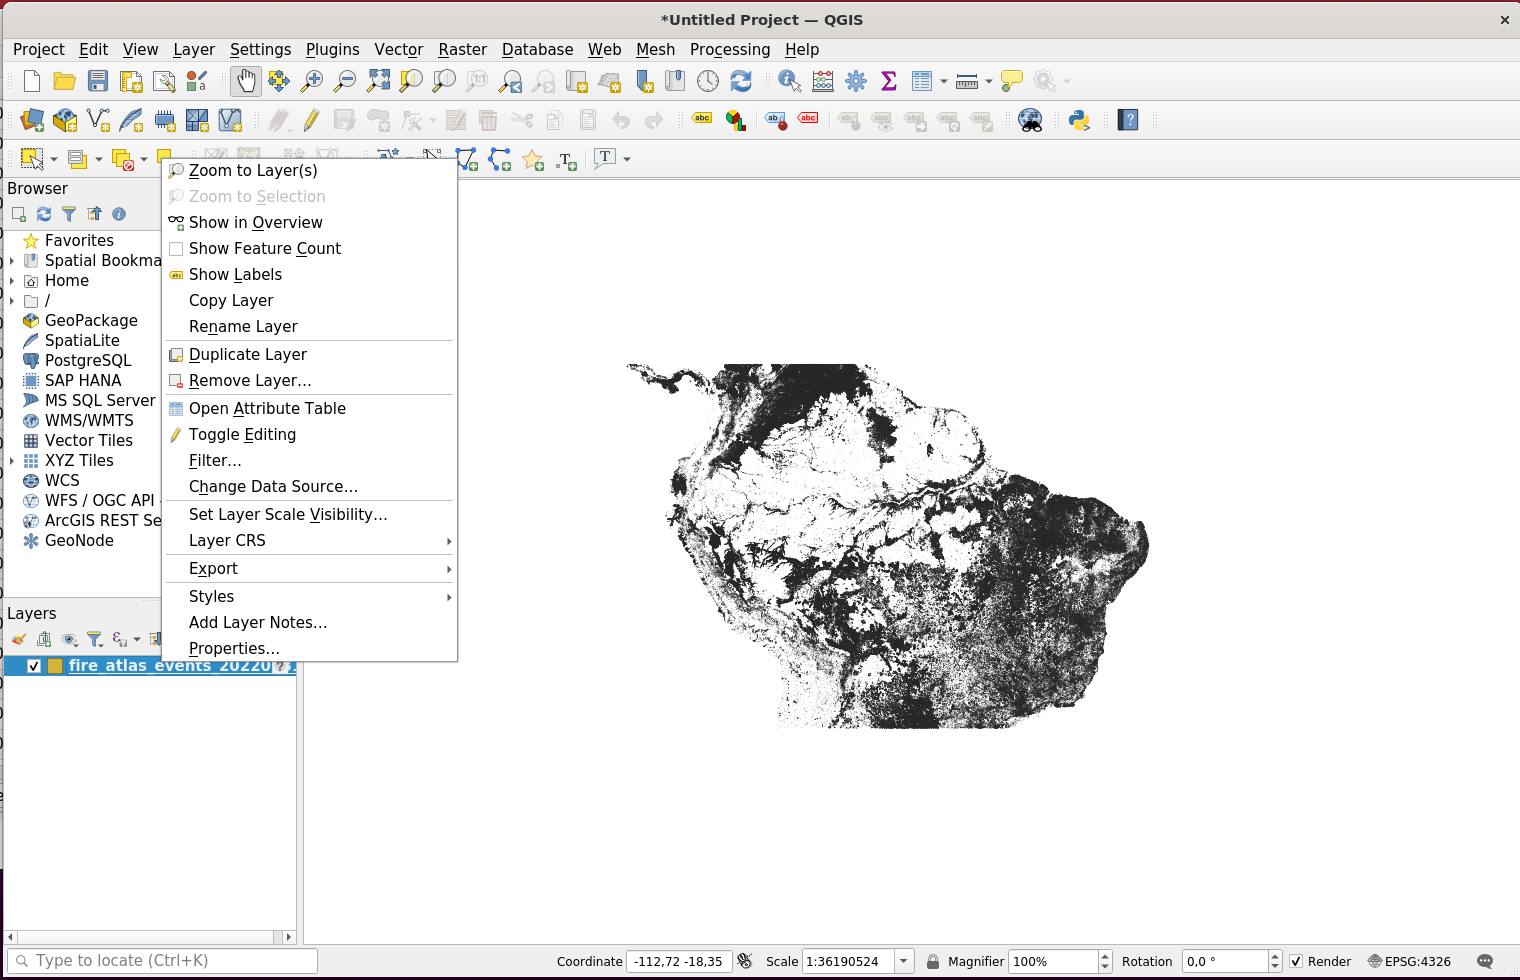
\includegraphics[width=\linewidth]{tg1/figuras/mapa.png}
		\caption{Mapa da América do Sul com os eventos de fogo detectados} \label{fig:mapashp}
	\end{minipage}
\end{figure}

\begin{figure}[htb]
	\centering
	\begin{minipage}{0.9\linewidth}
		\centering
		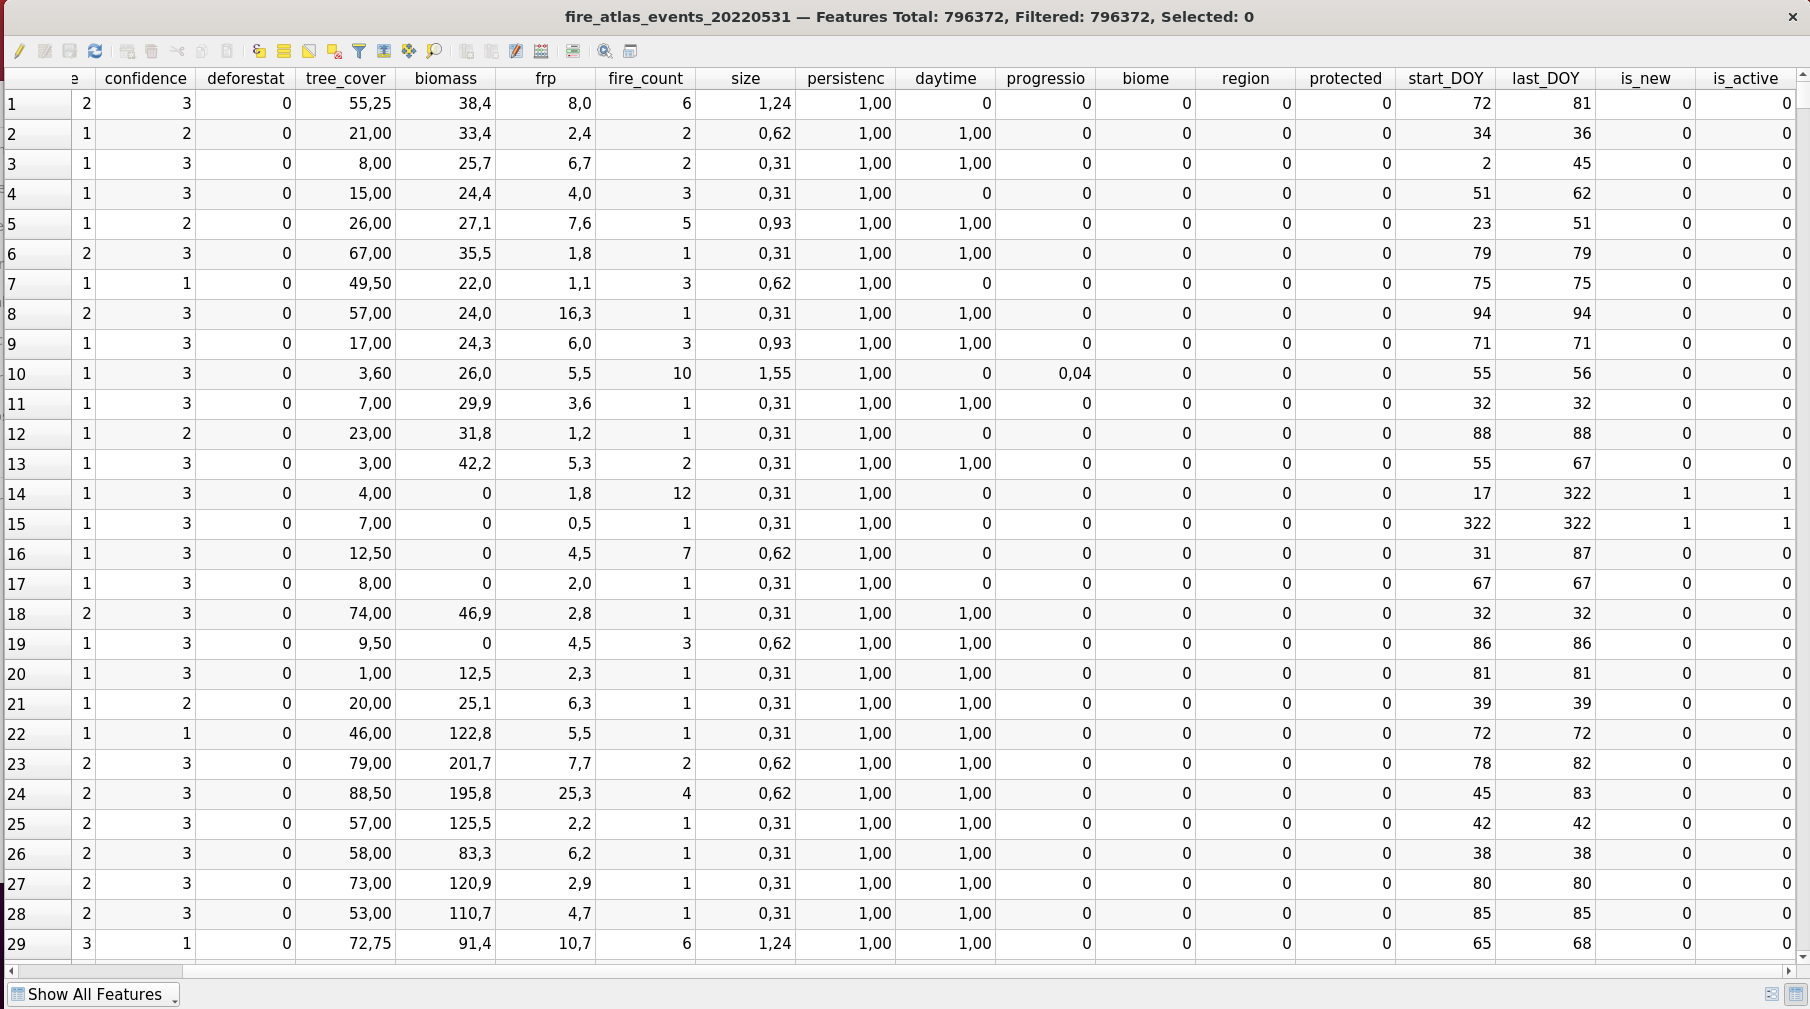
\includegraphics[width=\linewidth]{tg1/figuras/tabela_atributos.png}
		\caption{Tabela de atributos do \textit{shapefile}} \label{fig:tabat}
	\end{minipage}
\end{figure}

\newpage

\begin{multicols}{2}
    

\begin{itemize}
    \item \textbf{fire\_type:} tipo de fogo - (1) savana e pastagem, (2) pequenas clareiras, (3) sub-bosque, (4) desmatamento;
    \item \textbf{confidence:} confiança - (1) baixa, (2) moderada, (3) alta;
    \item \textbf{tree\_cover:} fração média de cobertura arbórea dentro do perímetro (\%);
    \item \textbf{biomass:} biomassa média dentro do perímetro do fogo (ton/ha);
    \item \textbf{deforestation:} fração (0-1) de quadrante de 550m com desmatamento histórico (2015-2019);
    \item \textbf{size:} tamanho do fogo em $km^2$;
    \item \textbf{detections:} número total de detecções dentro do período;
    \item \textbf{frp:} potência radiativa média de fogo (FRP) em megawatts (MW).  Trata-se de uma técnica para quantizar biomassa queimada medindo a radiação de energia infravermelha \cite{NASAMODIS};
    \item \textbf{persistence:} persistência em dias;
    \item \textbf{progression:} fração média de progressão do fogo em quadrantes de 550m (0-1);
    \item \textbf{daytime:} (0) não de dia, (1) de dia;
    \item \textbf{start\_DOY:} dia do início do novo incêndio a partir do dia do ano (1-366);
    \item \textbf{last\_DOY:} detecção de incêndio ativa mais recente a partir do dia do ano (1-366);
    \item \textbf{is\_new:} (1) começou nas últimas 24 horas, (0) incêndio já existente;
    \item \textbf{is\_active:} (1) o fogo estava ativo nos últimos 10 dias (0) ou não;
    \item \textbf{biome:} (1) o fogo está dentro (0) ou fora do bioma Amazônia;
    \item \textbf{protected:} fração (0-1) de fogo ocorrendo dentro de área protegida ou terra indígena;
    \item \textbf{region:} (0-21) qual a região do evento do fogo.
\end{itemize}
\end{multicols}

\subsection{\textit{Dataframe}}

Para converter o conteúdo da tabela de atributos em um \textit{dataframe}, faz-se necessário o uso das bibliotecas \textit{geopandas} e \textit{pandas} do \textit{python}. \textit{Pandas} é uma ferramenta de análise e manipulação de dados, e \textit{geopandas} estende os tipos de dados usados pelos \textit{pandas} para permitir operações espaciais em tipos geométricos. O que fazemos então é primeiro abrir o arquivo do tipo \textit{shapefile} usando \textit{geopandas} para criar um \textit{GeoDataFrame} e então usar uma função da biblioteca \textit{pandas} para convertê-lo em um \textit{dataframe} normal com as \textit{features} que iremos utilizar como entrada para os algoritmos de aprendizado de máquina.

\section{Censipam}
\label{sec:censipamBD}

Assim como o \textit{Amazon Dashboard}, o banco de dados obtido pelo Censipam está em formato \textit{shapefile}. Tal banco pode ser acessado através do recurso de adição de camadas Web Feature Service (WFS) no QGIS, utilizando uma URL específica que aponta para um serviço remoto contendo dados vetoriais geoespaciais. O WFS é um padrão da Open Geospatial Consortium (OGC) que define interfaces para servir e consumir dados geoespaciais vetoriais pela web.

Na figura \ref{fig:qgiscensipam} temos um exemplo do que podemos visualizar ao acessar o banco de dados do Censipam pelo QGIS:

\begin{figure}[htb]
	\centering
	\begin{minipage}{0.6\linewidth}
		\centering
		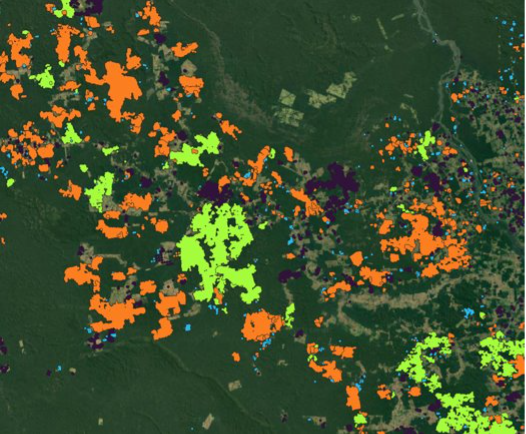
\includegraphics[width=\linewidth]{tg1/figuras/mapa_censipam.png}
		\caption{Mapa no QGIS com eventos de fogo} \label{fig:qgiscensipam}
	\end{minipage}
\end{figure}

Uma adição interessante presente nos dados do Censipam se comparados com os do GFED, é a capacidade de adquirirmos diversas detecções de um mesmo evento de fogo como demonstrado na figura \ref{fig:progressao}. Com o GFED tinhamos acesso apenas a classificação e \textit{features} mais recente do incêndio, referente a sua última detecção realizada, porém com o Censipam podemos obter ambos para detecções passadas, o que abre a possibilidade de incluir as características dinâmicas e temporais da queimada na sua classificação.



\begin{figure}[htb]
	\centering
	\begin{minipage}{0.9\linewidth}
		\centering
		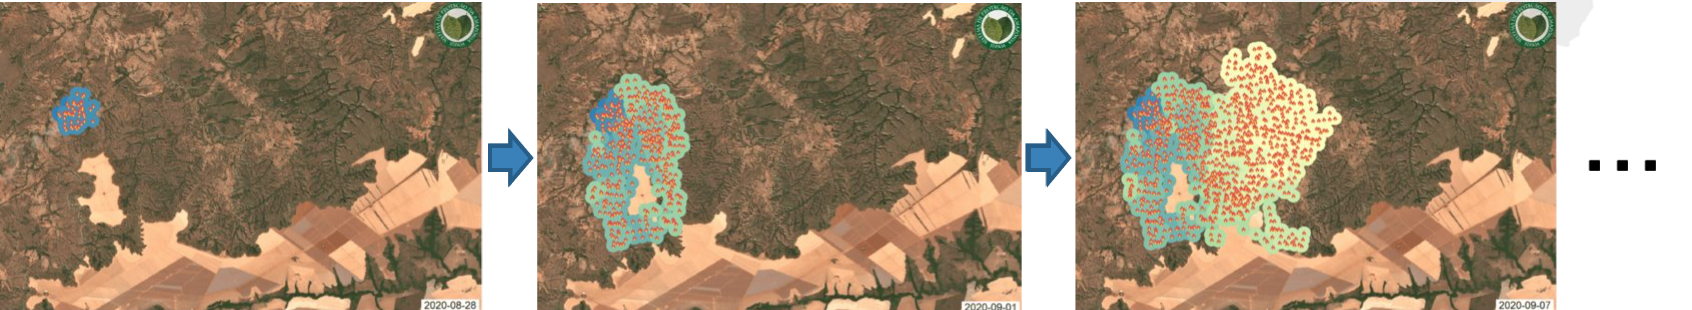
\includegraphics[width=\linewidth]{tg1/figuras/progressao_queimada.png}
		\caption{Ilustrações demonstrativas do crescimento de um evento de fogo ao longo do tempo} \label{fig:progressao}
	\end{minipage}
\end{figure}

Da tabela de atributos destes \textit{shapefiles}, utilizamos as seguintes colunas para o treinamento:

\newpage

\begin{multicols}{2}
    


\begin{itemize}
\item \textbf{id\_evento}: Representa o código de identificação interno de um evento de fogo catalogado pelo sistema. Detecções distintas mas consideradas como um mesmo evento recebem a mesma identificação.
\item \textbf{delta\_area}: Variação da área coberta pelo incêndio em kilometros quadrados.
\item \textbf{q\_focos}: Quantidade de focos de incêndio detectados pelo sistema como pertencendo ao mesmo evento de fogo.
\item \textbf{qtd\_passagens\_com\_deteccao}: Quantas passagens de satélites ocorreram por este evento. Como se trata de 4 pares de satélite em órbitas polares, pode-se ter até 8 detecções por dia \cite{painel-fogo}.
\item \textbf{frp\_med}: \textit{Fire Radiative Power} ou FRP, um dado relativo ao sensor MODIS (\textit{Moderate Resolution Imaging Spectroradiometer}).
\item \textbf{area\_passagem}: Área coberta pelo incêndio no momento da detecção;
\item \textbf{delta\_t\_horas}: Tempo acumulado em horas entre detecções.
%\item \textbf{p\_norm}:
\item \textbf{ve\_expansao}: Velocidade estimada de expansão do incêndio.

\end{itemize}

\end{multicols}

\section{Análise das \textit{features} do GFED}
\label{sec:features}

Ao todo são utilizadas 17 \textit{features} diferentes para realizarmos a classificação do tipo de fogo, que estão descritas na subseção \ref{sec:shp} (cluster\_ID não é utilizado). Nem sempre todas as informações que entregamos para um algoritmo de aprendizado de máquina são úteis para a previsão, o que explica não utilizarmos o cluster\_ID, pois se cada evento de fogo possui um número de identificação diferente, esse número nada diz a respeito sobre qual o tipo de queimada que ocorreu. Podemos fazer uma correlação entre cada tipo de dado fornecido e os tipos de fogo, observando assim quais informações são mais descritivas para o algoritmo, quais delas são mais úteis para separar os 4 tipos.

Para podermos observar a relação que cada \textit{feature} possui com a saída, foram feitos diversos gráficos de dispersão em 3 dimensões que combinam o efeito que até 3 \textit{features} em conjunto podem ter para separar cada tipo de queimada em nuvens. Os gráficos estão dispostos nas figuras a seguir:


\begin{multicols}{2}

\begin{figure}[H]
    \caption{Start day x Is new x Is active}
     
    \centering 
    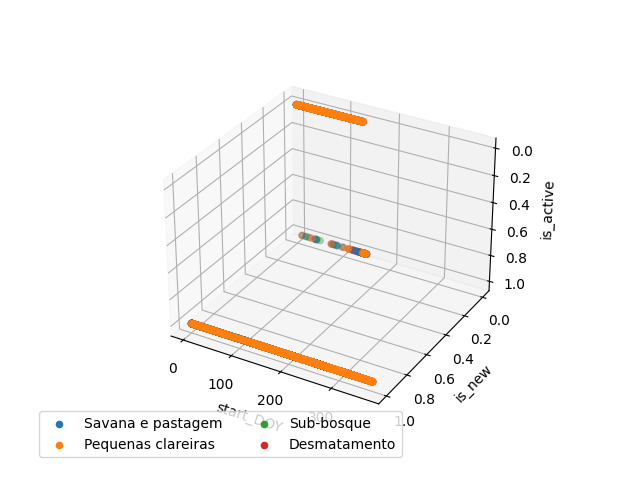
\includegraphics[width=0.9\linewidth]{tg1/figuras/start_DOYxis_newxis_active--150--120.png}
    \label{figura:six}
\end{figure}

\begin{figure}[H]
    \caption{Biome x Region x Protected}
     
    \centering 
    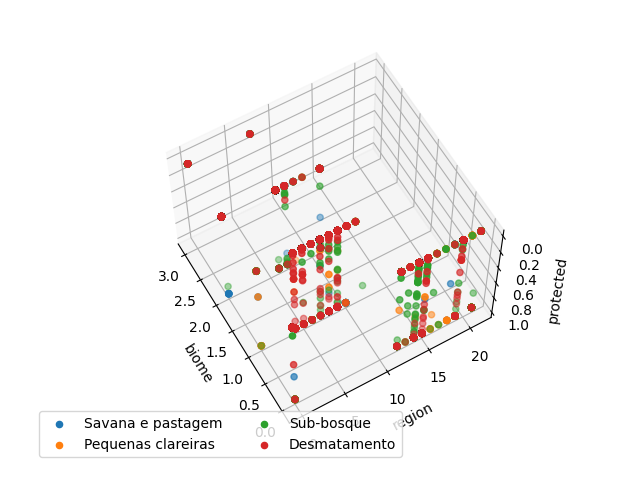
\includegraphics[width=1.1\linewidth]{tg1/figuras/biomexregionxprotected--120-30.png}
    \label{figura:one}
\end{figure}
        
\begin{figure}[H]
    \caption{Biome x Region x Protected}
     
    \centering 
    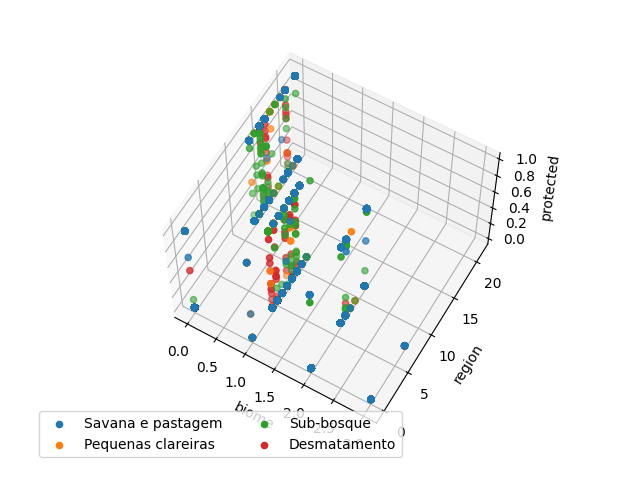
\includegraphics[width=1.1\linewidth]{tg1/figuras/biomexregionxprotected-60--60.png}
    \label{figura:two}
\end{figure}

\begin{figure}[H]
    \caption{Deforestat x Tree cover x Biomass}
     
    \centering 
    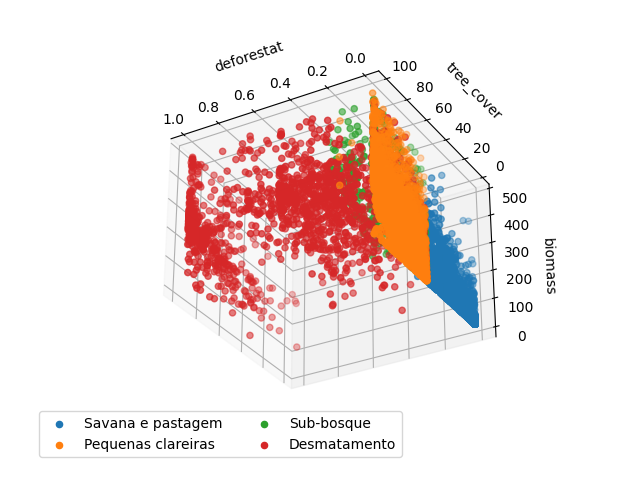
\includegraphics[width=1.1\linewidth]{tg1/figuras/deforestatxtree_coverxbiomass---30--120.png}
    \label{figura:three}
\end{figure}

\begin{figure}[H]
    \caption{FRP x Detections x Size}
     
    \centering 
    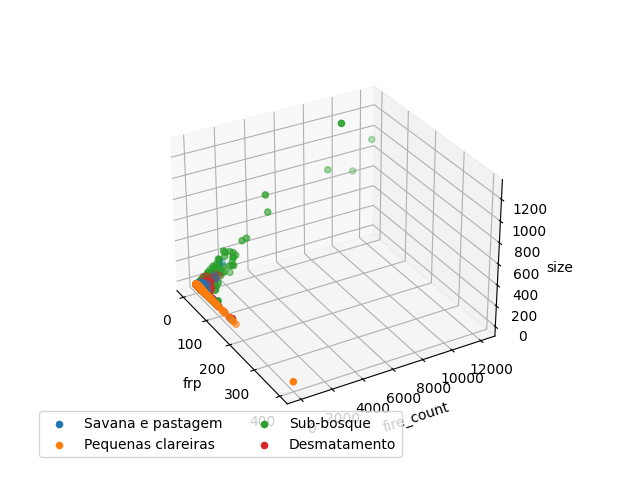
\includegraphics[width=1.1\linewidth]{tg1/figuras/frpxfire_countxsize-30--30.png}
    \label{figura:four}
\end{figure}

\begin{figure}[H]
    \caption{Persistence x Daytime x Progression}
     
    \centering 
    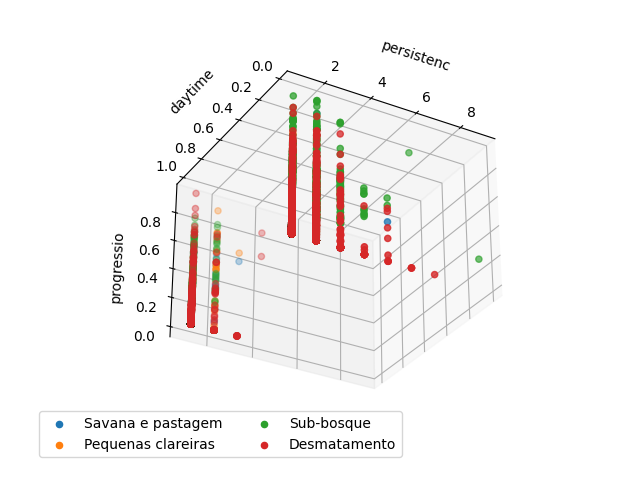
\includegraphics[width=1.1\linewidth]{tg1/figuras/persistencxdaytimexprogressio--30--120.png}
    \label{figura:five}
\end{figure}

\begin{figure}[H]
    \caption{Start day x Is new x Is active}
     
    \centering 
    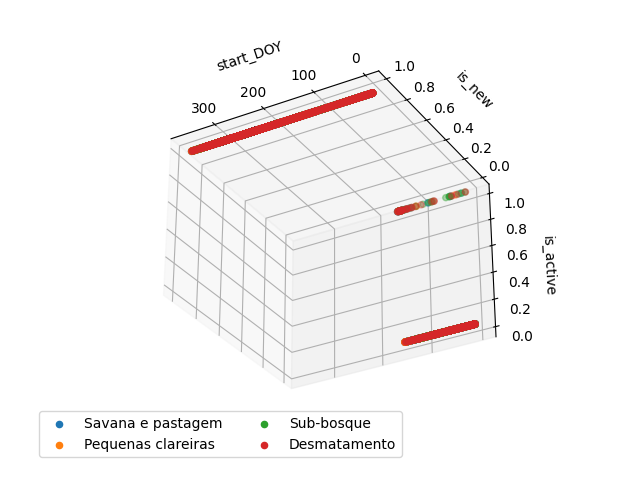
\includegraphics[width=1.1\linewidth]{tg1/figuras/start_DOYxis_newxis_active--30-120.png}
    \label{figura:seven}
\end{figure}
            
\end{multicols}

Podemos observar através dos gráficos que os tipos de fogo de savana (0) e pequenas clareiras (1) são mais fáceis de se tipificar, dados como \textit{tree cover}, \textit{deforestat}, \textit{frp}, \textit{fire count} e \textit{biomass} em conjunto são capazes de delimitar fortemente esses dois tipos. O desmatamento (4) e sub-bosque (3) apresentam maior diluição um com o outro e com os outros tipos, o que explica a maior dificuldade dos algoritmos em prevê-los corretamente, como será visto no capítulo \ref{resultados}.

Como podemos ver na seção \ref{sec:censipamBD}, o banco de dados do Censipam não conta com boa parte das \textit{features} presentes no banco do GFED, e como podemos ver algumas delas se mostraram essenciais para acusação do tipo do fogo. Torna-se necessário então buscar outras fontes que forneçam tais informações.

%\todo[inline]{}

\section{Adição de \textit{features}}
%Dos dados listados acima, apenas 18 são disponibilizados diretamente pelos servidores do CENSIPAM. Os demais dados têm de ser produzidos a partir de outros conjuntos de dados disponibilizados por diferentes entidades. 

A produção destes dados para a adição ao banco do Censipam envolve o cruzamento com dados de diversas outras entidades. Sua produção se dá pelo cálculo da intersecção geográfica dos eventos de fogo e diversos mapas disponibilizadas pelas entidades Terrabrasilis \cite{terrabrasilis}, MapBiomas \cite{MapBiomasQueimadas} e GFED \cite{gfed}.

A partir das coordenadas dos focos de incêndio, é possível de se fazer uma comparação com outros mapas para se encontrar intersecções com áreas de interesse. Por exemplo, dados relativos à proximidade à áreas de conservação ambiental e áreas indígenas são produzidos pelo cruzamento com os dados disponíveis pelo Terrabrasilis. Já informações como desmatamento da área podem ser obtidas por meio do DETER \cite{deter}, enquanto informações Áreas Públicas, Privadas, Desconhecidas e Áreas de Cadastro Ambiental Rural são obtidas a partir do Cadastro Ambiental Rural \cite{cadastro-rural}.

 O código de aquisição e cruzamento foi feito com base no modelo desenvolvido por Bruno Scholles \cite{BrunoScholess2023}, por meio do qual foi-se possível adicionarmos as seguintes \textit{features} ao \textit{dataframe}:

\begin{figure}[htb]
	\centering
	\begin{minipage}{0.9\linewidth}
		\centering
		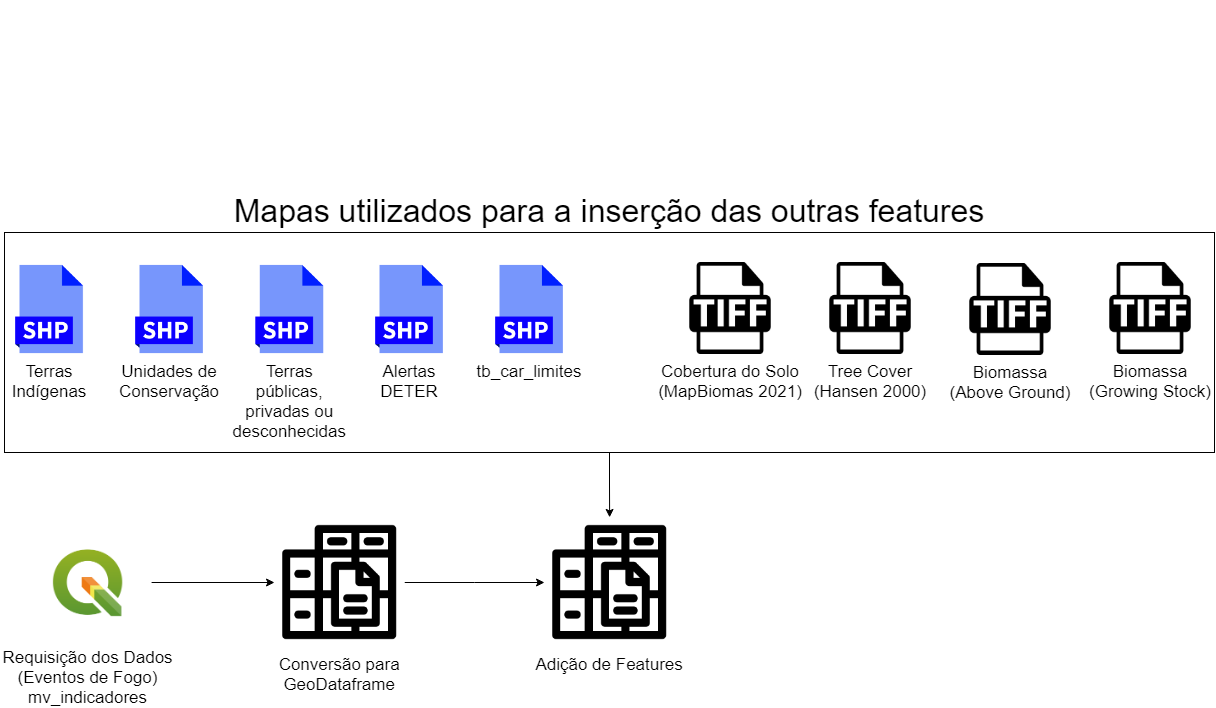
\includegraphics[width=\linewidth]{tg1/figuras/esquematico_banco.png}
		\caption{Esquemático do processo de obtenção de \textit{features}} \label{fig:featuresextras}
	\end{minipage}
\end{figure}
\begin{multicols}{2}
    \begin{itemize}
\item \textbf{areakm2\_UC}: Área em $km^2$ da detecção pertencente à uma unidade de conservação;
\item \textbf{perc\_in\_UC}: Porcentagem da área da detecção da detecção pertencente à uma unidade de conservação;
\item \textbf{areakm2\_IN}:Área em $km^2$ da detecção pertencente à território indígena;
\item \textbf{perc\_in\_IN}:Porcentagem da área da detecção da detecção pertencente à território indígena;
\item \textbf{deter\_area}:Área em $km^2$ da detecção pertencente à área em que ocorreu desmatamento;
\item \textbf{deter\_days}: Quantidade de dias passados desde a demarcação do DETER como área em que ocorreu desmatamento; 
\item \textbf{deter\_perc}:Porcentagem da área da detecção da detecção pertencente à área em que ocorreu desmatamento;
\item \textbf{tree\_cover}: Cobertura de árvore, métrica referente à porcentagem da área que é coberta por copas de árvores ou vegetação alta.
\item \textbf{a\_cover\_X e p\_cover\_X (onde X pode ser 3, 4, 5, 9, 11, 12, 15, 20, 21, 23, 24, 25, 29, 30, 32, 33, 39, 40, 41, 48, 62)}: Cobertura do solo (tipo de vegetação) medida em área e porcentagem;
\item \textbf{biomass\_AG}: biomassa \textit{Above Ground} média dentro do perímetro
\item \textbf{biomass\_GS}: biomassa \textit{Growing Stock} média dentro do perímetro
\item \textbf{a\_terr\_pri e p\_terr\_pri}: Perímetro da detecção pertencente à área privada;
\item \textbf{a\_terr\_pub e p\_terr\_pub}: Perímetro da detecção pertencente à área pública;
\item \textbf{a\_terr\_unk e p\_terr\_unk}: Perímetro da detecção pertencente à área não classificada como pública ou privada (\textit{unknown});
\item \textbf{area\_CAR e per\_car}: Perímetro da detecção pertencente à área de Cadastro Ambiental Rural;
\end{itemize}
\end{multicols}




